\chapter{Getting started}

This file describes the ILLC Dissertation Style package for
typesetting dissertations in \LaTeX\ according to ILLC standards.
It describes which files are needed, and how they should be adopted
for your dissertation.
It also serves as an example of using these files, and as a template
for your own dissertation.

The ILLC Dissertation Style file will change the
layout of your dissertation to the required ILLC Dissertation Style.
It defines a standard layout for the cover and spine of your dissertation,
and includes a list of previous publications in the ILLC Dissertation series
Furthermore, it redefines the layout of \verb|\chapter|, page heads,
and theorem-like environments,
and provides predefined theorem-like environments and
commands for special sections such as \verb|\acknowledgements|.

If you are already familiar with the standard {\tt book.cls} provided with
\LaTeX 2$\epsilon$, then the ILLC Dissertation Style file should not give you
any difficulties: you may use all {\tt book} style commands to prepare 
your dissertation.
For a description of the commands available in the \LaTeX 2$\epsilon$\ 
{\tt book} style we refer you to the {\em \LaTeX{} User's Guide \& Reference
Manual\/} by Leslie Lamport (1986, 1994), Addison-Wesley Publishing
Company, Reading, Mass.

\section{How to proceed}
The complete ILLC Dissertation Style package contains the following files:
\begin{description} 
\item[{\tt illcdiss.cls}:] the ILLC Dissertation Style for
use with \LaTeX 2$\epsilon$
\item[{\tt illcdissertations.tex}:] file containing data on previous
  ILLC Dissertations
\item[{\tt illclogo.eps}:] this is the ILLC logo;
  input by {\tt guide\_front.tex}
\item[{\tt illc\_no\_text\_logo.eps}:] the ILLC logo without text;
  input by {\tt guide\_spine.tex}
\item[{\tt illclogo.pdf}, {\tt illc\_no\_text\_logo.pdf}:] PDF versions of the logos, used by {\tt pdflatex} instead of the EPS versions
\item[{\tt guide.tex}:] the main latex file for this document
\item[{\tt guide\_front.tex}:] file describing the official 
  ILLC-Dissertation front matter
\item[{\tt titlepage\_from\_pedel.pdf}:] placeholder for the title page which you will receive from the Bureau Pedel (Office of the Beadle)
\item[{\tt guide\_XXX.tex}:] file containing the text of section XXX of this 
document
\item[{\tt guide\_spine.tex}:] file for preparing the text 
  for the spine of your dissertation
\end{description}
You should make sure that \LaTeX\ is able to find the files
{\tt illcdissertations.tex}, {\tt illcdiss.cls}, {\tt illclogo.eps} and
{\tt illc\_no\_text\_logo.eps} when you 
typeset your document with the ILLC Dissertation Style; one way
to achieve this is to put all files in the ILLC Dissertation Style
package in the directory (or folder) where your dissertation files
reside.

Note that the {\tt illcdissertations.tex}
file in the archive is automatically updated for any new dissertations:
please download the most recent version 
before sending your dissertation to the printers.

\section{Invoking the ILLC Dissertation Style}
The ILLC Dissertation Style is invoked by replacing ``book'' by ``illcdiss''
in the first line of your document. You should also \verb|\include| 
a {\em personalized\/} version of the file {\tt guide\_front.tex} 
after the \verb|\begin{document}| declaration. 
You also need to \verb|\include| the file
\verb|illcdissertations.tex| after the last page of your dissertation:

\begin{verbatim}
\documentclass{illcdiss}

\begin{document}
\pagestyle{plain}
\pagenumbering{roman}

%%  \include the `front matter'

%% This is the standard `front matter' to be used with the illcdiss.cls
%% Latex2e document class
%%
%% Author: Maarten de Rijke
%% Current maintainer: Marco Vervoort
%%
%% Version: July, 2001
%%
%%
%% Amendment August, 2020 by Gianluca Grilletti: the nationality of the candidate should not be indicated in the titelblad, independently from the birth country
%%
%%
%%
%% MAKE SURE THAT THE FILE HAS BEEN PERSONALIZED BEFORE YOU
%% PRINT AND SHIP THE FINAL VERSION.  YOU CAN FIND ITEMS THAT NEED
%% TO BE PERSONALIZED BY SEARCHING FOR THE STRING ``%PERSONALIZE''
%%
%%
%%first of all the cover.
{\pagestyle{empty}
\newcommand{\printtitle}{%
{\Huge\bfseries The ILLC Dissertation\\[0.8cm] Style}}    %PERSONALIZE

\begin{titlepage}
\par\vskip 2cm
\begin{center}
\printtitle
\vfill
{\LARGE\bfseries John B. Goode}                           %PERSONALIZE
\vskip 2cm
\end{center}
\end{titlepage}
%
% Skip a page to start on a right page again.
% If you're printing single-sided, simply delete    %PERSONALIZE
% the following line.
%
\mbox{}\newpage
\setcounter{page}{1}

%%the very first page: the `franse pagina'
\par\vskip 2cm
\begin{center}
\printtitle
\end{center}

%%the second page: the `illc pagina'
\clearpage
\par\vskip 2cm
\begin{center}
ILLC Dissertation Series DS-200X-NN                 %PERSONALIZE
\par\vspace {2cm}
\illclogo{10cm}
\par\vspace {2cm}
\noindent%
For further information about ILLC-publications, please contact\\[2ex]
Institute for Logic, Language and Computation\\
Universiteit van Amsterdam\\
Science Park 107\\
1098 XG Amsterdam\\
phone: +31-20-525 6051\\
e-mail: {\tt illc@uva.nl}\\
homepage: {\tt http://www.illc.uva.nl/}
\end{center}
\vfill

% If you're supported by NWO adapt the following 6 lines;
% otherwise simply delete them.
%
\noindent%
The investigations were supported by the            %PERSONALIZE
Philosophy Research Foundation\linebreak (SWON), 
which is subsidized by the Netherlands 
Organization for Scientific\linebreak Research (NWO).
\par\vspace {2cm}

% If you want to add CIP data (a summary of all the data used in
% library catalogs in a standard format), uncomment the following
% three lines and add the CIP data in between
%
%\noindent%
%{\tt CIP gegevens}                                 % PERSONALIZE
%\\[4ex]                                            %PERSONALIZE

%Copyright and accreditation stuff, plus ISBN
%
\noindent%
% Copyright: put your name here
Copyright \copyright\ 200X by John B.\ Goode\\[2ex] %PERSONALIZE
% Cover design, if your cover was designed by someone else
Cover design by Bert Jones.\\                       %PERSONALIZE
%Maybe some additional info on the production of the dissertation.
%Don't forget your printing shop
Printed and bound by your printer.\\[2ex]           %PERSONALIZE
%ISBN number: ask your printing shop to obtain one for you
ISBN: 90--XXXX--XXX--X                              %PERSONALIZE

% Dedication, table of contents and acknowledgements
% are handled in the main file


%%the third and fourth page, the `titelblad' and promotores-list, will be sent to you by the Pedel. Replace the file 'titlepage_from_pedel.pdf' by what you receive.
\clearpage
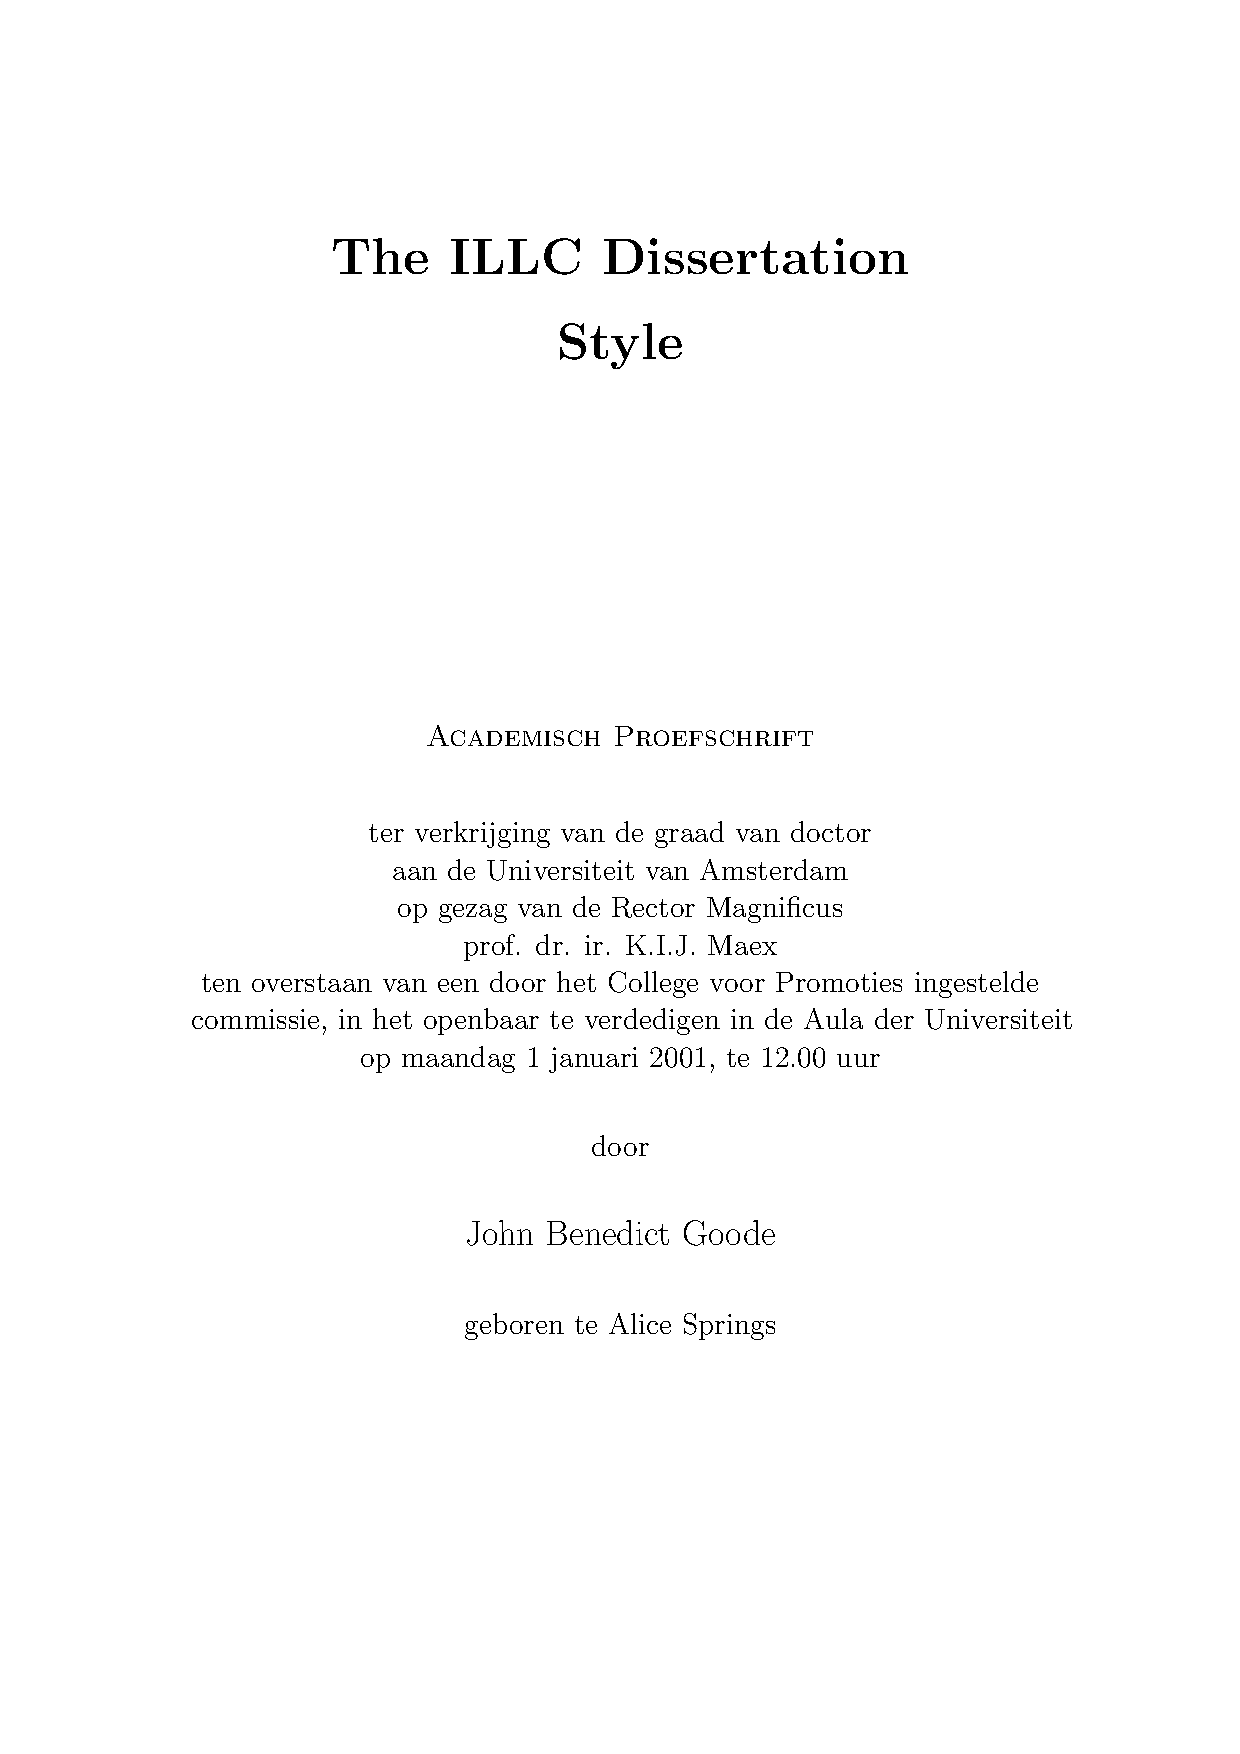
\includepdf[pages={1,2}]{titlepage_from_pedel.pdf}
%%Formerly the pages were generated by the following content
%  \par\vskip 2cm
%  \begin{center}
%  \printtitle
%  \par\vspace {6cm}
%  {\large \sc Academisch Proefschrift}
%  \par\vspace {1cm}
%  {\large ter verkrijging van de graad van doctor\\
%  aan de Universiteit van Amsterdam\\
%  op gezag van de Rector Magnificus\\
%  prof. dr. ir. K.I.J. Maex\\                                 %PERSONALIZE
%  ten overstaan van een door het College voor Promoties ingestelde\\
%  \mbox{commissie, in het openbaar te verdedigen in de Aula der Universiteit}\\        %PERSONALIZE
%  % Note: If your UvA PhD defense is located at the Agnietenkapel, simply write
%  % 'te verdedigen in de Agnietenkapel \\', i.e. do not add 'der Universiteit'
%  op maandag 1 januari 2001, te 12.00 uur \\ }        %PERSONALIZE
%  \par\vspace {1cm} {\large door}
%  \par \vspace {1cm} % Note: next should be your _full_ name
%  {\Large John Benedict Goode}                        %PERSONALIZE
%  \par\vspace {1cm} % and your birthplace
%  {\large geboren te Alice Springs} %PERSONALIZE
%  % Note: NEVER include your country of birth, only the city of birth
%  \end{center}
%  \clearpage
%  \noindent%
%  {\bfseries Promotiecommissie}\\
%  \\
%  \begin{tabular}[t]{@{}llr}
%  Promotor:      & Prof.dr.\ J.~Smith  & Universiteit van Amsterdam \\  %PERSONALIZE
%  Co-promotor:   & Dr.\ T.~Jones       & Universiteit van Amsterdam \\  %PERSONALIZE
%  \\
%  Overige leden: & Prof. Dr. A. Aap    & Universiteit van Amsterdam \\  %PERSONALIZE
%                 & Prof. Dr. B. Benson & Universiteit van Amsterdam \\  %PERSONALIZE
%                 & Dr. C. Cornelissen  & Universiteit van Amsterdam \\  %PERSONALIZE
%  \end{tabular}\\
%  \\
%  Faculteit der Natuurwetenschappen, Wiskunde en Informatica\\ %PERSONALIZE

\clearpage
} % Back to \pagestyle{plain}

%%%%%%%%%%%%%%%%%%%%%%%END of FRONT MATTER%%%%%%%%%%%%%%%%%%%%%%%%%%%

\thispagestyle{plain}
\mbox{}
\vspace{2in}
\begin{center}
{\em to me \\ \ \\
who did all the work on this}
\footnote{The dedication is optional}
\end{center}

\tableofcontents
\acknowledgments

I am very grateful to Prof.dr.\ J.\ Smith whose help proved really extremely
invaluable.\\[2ex]				
Alice Springs\hfill John B. Goode\\
October, 200X.



%%  now we can start with the real thing

\cleardoublepage
\pagestyle{headings}
\pagenumbering{arabic}
  
    <your dissertation>

%%  \include the `end matter'

% \begin{thebibliography}{XX}
% \bibitem{Comment}
% According to ILLC standards a chapter containing bibliographic
% references should always be included in your dissertation.
% It is specified by:
% \begin{verbatim}
%   \begin{thebibliography}{XX}
%     <your list of \bibitems>
%   \end{thebibliography}
% \end{verbatim}
% \bibitem{Lamport}
% L. Lamport. {\em \LaTeX{} User's Guide \& Reference
% Manual\/}, Addison-Wesley Publishing Company, Reading, Mass. 1986, 1994.
% \end{thebibliography}

\bibliography{biblio}


\begin{theindex}
By preference, your dissertation\linebreak
should contain an index. Instructions
on how to produce an index can be
found on pages 77--79 of the
 \LaTeX\ manual. You may specify
an index as follows:\\[2ex]
\verb|  \begin{theindex}|\\
\verb|    <your list of entries>|\\
\verb|  \end{theindex}|
\end{theindex}


\begin{thesymbols}
This is an optional chapter containing a list of symbols that
you use. It is specified by:\\[2ex]
\verb|  \begin{thesymbols}|\\
\verb|    <your list of symbols>|\\
\verb|  \end{thesymbols}|
\end{thesymbols}

\samenvatting
According to both ILLC standards and UvA promotion regulations,
a chapter containing a summary in
Dutch of your dissertation should always be included.
It is specified by:
\begin{verbatim}
  \samenvatting
    <your Samenvatting>
\end{verbatim}

\abstract
According to both ILLC standards and UvA promotion regulations,
an abstract of your dissertation in English should always be included.
This chapter may be specified by:
\begin{verbatim}
  \abstract
    <your Abstract>
\end{verbatim}


\curriculum
This is an optional chapter containing your Curriculum Vitae.
It is specified as follows:
\begin{verbatim}
  \curriculum
    <your CV>
\end{verbatim}



%%  finally, \include the list of previous ILLC dissertations

\pagestyle{empty}

\noindent
{\em Titles in the ILLC Dissertation Series:}

\newcommand{\illcpublication}[3]{\item[ILLC #1: ]{\bfseries #2}\\{\em #3}}

\begin{list}{}{ \settowidth{\leftmargin}{ILL}
		\setlength{\rightmargin}{0in}
		\setlength{\labelwidth}{\leftmargin}
		\setlength{\labelsep}{0in}
}

\illcpublication{DS-2016-01}{Ivano A. Ciardelli}{Questions in Logic}
\illcpublication{DS-2016-02}{Zoé Christoff}{Dynamic Logics of Networks: Information Flow and the Spread of Opinion}
\illcpublication{DS-2016-03}{Fleur Leonie Bouwer}{What do we need to hear a beat? The influence of attention, musical abilities, and accents on the perception of metrical rhythm}
\illcpublication{DS-2016-04}{Johannes Marti}{Interpreting Linguistic Behavior with Possible World Models}
\illcpublication{DS-2016-05}{Phong Lê}{Learning Vector Representations for Sentences - The Recursive Deep Learning Approach}
\illcpublication{DS-2016-06}{Gideon Maillette de Buy Wenniger}{Aligning the Foundations of Hierarchical Statistical Machine Translation}
\illcpublication{DS-2016-07}{Andreas van Cranenburgh}{Rich Statistical Parsing and Literary Language}
\illcpublication{DS-2016-08}{Florian Speelman}{Position-based Quantum Cryptography and Catalytic Computation}
\illcpublication{DS-2016-09}{Teresa Piovesan}{Quantum entanglement: insights via graph parameters and conic optimization}
\illcpublication{DS-2016-10}{Paula Henk}{Nonstandard Provability for Peano Arithmetic. A Modal Perspective}
\illcpublication{DS-2017-01}{Paolo Galeazzi}{Play Without Regret}
\illcpublication{DS-2017-02}{Riccardo Pinosio}{The Logic of Kant's Temporal Continuum}
\illcpublication{DS-2017-03}{Matthijs Westera}{Exhaustivity and intonation: a unified theory}
\illcpublication{DS-2017-04}{Giovanni Cinà}{Categories for the working modal logician}
\illcpublication{DS-2017-05}{Shane Noah Steinert-Threlkeld}{Communication and Computation: New Questions About Compositionality}
\illcpublication{DS-2017-06}{Peter Hawke}{The Problem of Epistemic Relevance}
\illcpublication{DS-2017-07}{Aybüke Özgün}{Evidence in Epistemic Logic: A Topological Perspective}
\illcpublication{DS-2017-08}{Raquel Garrido Alhama}{Computational Modelling of Artificial Language Learning: Retention, Recognition \& Recurrence}
\illcpublication{DS-2017-09}{Miloš Stanojević}{Permutation Forests for Modeling Word Order in Machine Translation}
\illcpublication{DS-2018-01}{Berit Janssen}{Retained or Lost in Transmission? Analyzing and Predicting Stability in Dutch Folk Songs}
\illcpublication{DS-2018-02}{Hugo Huurdeman}{Supporting the Complex Dynamics of the Information Seeking Process}
\illcpublication{DS-2018-03}{Corina Koolen}{Reading beyond the female: The relationship between perception of author gender and literary quality}
\illcpublication{DS-2018-04}{Jelle Bruineberg}{Anticipating Affordances: Intentionality in self-organizing brain-body-environment systems}
\illcpublication{DS-2018-05}{Joachim Daiber}{Typologically Robust Statistical Machine Translation: Understanding and Exploiting Differences and Similarities Between Languages in Machine Translation}
\illcpublication{DS-2018-06}{Thomas Brochhagen}{Signaling under Uncertainty}
\illcpublication{DS-2018-07}{Julian Schlöder}{Assertion and Rejection}
\illcpublication{DS-2018-08}{Srinivasan Arunachalam}{Quantum Algorithms and Learning Theory}
\illcpublication{DS-2018-09}{Hugo de Holanda Cunha Nobrega}{Games for functions: Baire classes, Weihrauch degrees, transfinite computations, and ranks}
\illcpublication{DS-2018-10}{Chenwei Shi}{Reason to Believe}
\illcpublication{DS-2018-11}{Malvin Gattinger}{New Directions in Model Checking Dynamic Epistemic Logic}
\illcpublication{DS-2018-12}{Julia Ilin}{Filtration Revisited: Lattices of Stable Non-Classical Logics}
\illcpublication{DS-2018-13}{Jeroen Zuiddam}{Algebraic complexity, asymptotic spectra and entanglement polytopes}
\illcpublication{DS-2019-01}{Carlos Vaquero}{What Makes A Performer Unique? Idiosyncrasies and commonalities in expressive music performance}
\illcpublication{DS-2019-02}{Jort Bergfeld}{Quantum logics for expressing and proving the correctness of quantum programs}
\illcpublication{DS-2019-03}{András Gilyén}{Quantum Singular Value Transformation \& Its Algorithmic Applications}
\illcpublication{DS-2019-04}{Lorenzo Galeotti}{The theory of the generalised real numbers and other topics in logic}
\illcpublication{DS-2019-05}{Nadine Theiler}{Taking a unified perspective: Resolutions and highlighting in the semantics of attitudes and particles}
\illcpublication{DS-2019-06}{Peter T.S. van der Gulik}{Considerations in Evolutionary Biochemistry}
\illcpublication{DS-2019-07}{Frederik Möllerström Lauridsen}{Cuts and Completions: Algebraic aspects of structural proof theory}
\illcpublication{DS-2020-01}{Mostafa Dehghani}{Learning with Imperfect Supervision for Language Understanding}
\illcpublication{DS-2020-02}{Koen Groenland}{Quantum protocols for few-qubit devices}
\illcpublication{DS-2020-03}{Jouke Witteveen}{Parameterized Analysis of Complexity}
\illcpublication{DS-2020-04}{Joran van Apeldoorn}{A Quantum View on Convex Optimization}
\illcpublication{DS-2020-05}{Tom Bannink}{Quantum and stochastic processes}
\illcpublication{DS-2020-06}{Dieuwke Hupkes}{Hierarchy and interpretability in neural models of language processing}
\illcpublication{DS-2020-07}{Ana Lucia Vargas Sandoval}{On the Path to the Truth: Logical \& Computational Aspects of Learning}
\illcpublication{DS-2020-08}{Philip Schulz}{Latent Variable Models for Machine Translation and How to Learn Them}
\illcpublication{DS-2020-09}{Jasmijn Bastings}{A Tale of Two Sequences: Interpretable and Linguistically-Informed Deep Learning for Natural Language Processing}
\illcpublication{DS-2020-10}{Arnold Kochari}{Perceiving and communicating magnitudes: Behavioral and electrophysiological studies}
\illcpublication{DS-2020-11}{Marco Del Tredici}{Linguistic Variation in Online Communities: A Computational Perspective}
\illcpublication{DS-2020-12}{Bastiaan van der Weij}{Experienced listeners: Modeling the influence of long-term musical exposure on rhythm perception}
\illcpublication{DS-2020-13}{Thom van Gessel}{Questions in Context}
\illcpublication{DS-2020-14}{Gianluca Grilletti}{Questions \& Quantification: A study of first order inquisitive logic}
\illcpublication{DS-2020-15}{Tom Schoonen}{Tales of Similarity and Imagination. A modest epistemology of possibility}
\illcpublication{DS-2020-16}{Ilaria Canavotto}{Where Responsibility Takes You: Logics of Agency, Counterfactuals and Norms}
\illcpublication{DS-2020-17}{Francesca Zaffora Blando}{Patterns and Probabilities: A Study in Algorithmic Randomness and Computable Learning}
\illcpublication{DS-2021-01}{Yfke Dulek}{Delegated and Distributed Quantum Computation}
\illcpublication{DS-2021-02}{Elbert J. Booij}{The Things Before Us: On What it Is to Be an Object}
\illcpublication{DS-2021-03}{Seyyed Hadi Hashemi}{Modeling Users Interacting with Smart Devices}
\illcpublication{DS-2021-04}{Sophie Arnoult}{Adjunction in Hierarchical Phrase-Based Translation}
\illcpublication{DS-2021-05}{Cian Guilfoyle Chartier}{A Pragmatic Defense of Logical Pluralism}
\illcpublication{DS-2021-06}{Zoi Terzopoulou}{Collective Decisions with Incomplete Individual Opinions}
\illcpublication{DS-2021-07}{Anthia Solaki}{Logical Models for Bounded Reasoners}
\illcpublication{DS-2021-08}{Michael Sejr Schlichtkrull}{Incorporating Structure into Neural Models for Language Processing}
\illcpublication{DS-2021-09}{Taichi Uemura}{Abstract and Concrete Type Theories}
\illcpublication{DS-2021-10}{Levin Hornischer}{Dynamical Systems via Domains: Toward a Unified Foundation of Symbolic and Non-symbolic Computation}

\end{list}

\end{document}
\end{verbatim}
%
%
If your file is already coded with \LaTeX{} you can easily
adapt it a posteriori to the ILLC Dissertation Style.

If your document is coded with the ILLC Dissertation Style,
you may not be able to typeset it using the standard \LaTeX\ book style
without doing some minor recoding,
as the ILLC Dissertation Style file defines some comands 
that are not provided by the standard \LaTeX\ book style.

Please refrain from using any \LaTeX{} or \TeX{} commands
that affect the layout or formatting of your document
(i.e.\ commands like \verb|\textheight|, \verb|\hoffset| etc.).
The ILLC Dissertation Style has been carefully designed 
to produce the rightlayout from your \LaTeX\ input.
There may nevertheless be exceptional occasions on which to use some of them.
If there is anything specific you would like to do 
and for which neither \LaTeX{} nor the ILLC Dissertation Style file 
provides a command,
{\em please contact us\/} (email: illc@uva.nl).

\section{Personalizing {\tt guide\_front.tex}}
The file {\tt guide\_front.tex} contains all information needed 
to produce the front matter of your dissertation according to ILLC standards.
You need to personalize {\tt guide\_front.tex} by inserting your data
at appropriate spots. Additionally, those that print on single-sided
printers will want to eliminate the empty page printed after the cover page.
All items that need to be personalized in 
{\tt guide\_front.tex} can be found by searching for the string 
``\%{}PERSONALIZE''.

You will receive a version containing a title page from the Bureau Pedel (Office of the Beadle) once your dissertation has been approved by the committee.
This should be included as pages (iii) and (iv) of the front matter, using the pdfpages \verb|\includepdf| command.
An example file 'titlepage\_from\_pedel.pdf' is included with the style files.
Note that you may wish to temporarily comment out the \verb|\includepdf| command for the version that is sent to your committee, as at that point you will not yet have obtained the proper title page and the example file will list the wrong title.

The files {\tt guide\_dedication} and {\tt guide\_acknowledgements} 
contain the optional dedication and acknowledgements, and are \verb|\include|d
from the main file.
You can personalize the text in these files, or simply change the name
of the \verb|\include|d files in the main file.

\section{Personalizing {\tt guide\_spine.tex}}
The file {\tt guide\_spine.tex} contains all information needed
to produce the spine of your dissertation according to ILLC standards.
You need to personalize the file {\tt guide\_spine.tex} by inserting 
your data at appropriate spots. All items that need to be personalized in
{\tt guide\_spine.tex} can be found by searching for the string
``\%{}PERSONALIZE''.
